\documentclass[cs4size,a4paper,10pt]{ctexart}   

\linespread{1.5}
\usepackage{geometry}%用于设置上下左右页边距
	\geometry{left=2.5cm,right=2.5cm,top=3.2cm,bottom=2.7cm}
\usepackage{xeCJK,amsmath,paralist,enumerate,booktabs,multirow,graphicx,subfig,setspace,listings,lastpage,hyperref}
\usepackage{amsthm, amssymb, bm, color, framed, graphicx, hyperref, mathrsfs}
\usepackage{mathrsfs}  
	\setlength{\parindent}{2em}
	\lstset{language=Matlab}%
\usepackage{fancyhdr}
\usepackage{graphicx}
\usepackage{subfloat}
\usepackage{listings}
\usepackage{xcolor}
\usepackage{float}
\usepackage{paralist}
\usepackage{setspace}
\usepackage{titlesec}
\usepackage{enumitem}
\usepackage{hyperref}
\usepackage{multirow}
\usepackage{threeparttable}
\usepackage{autobreak}
\usepackage{multicol}
\usepackage{subfig}
\usepackage{unicode-math}
\usepackage{ltxtable, filecontents}
\usepackage{array}

\hypersetup{
	colorlinks=true,
	linkcolor=black,
	urlcolor=black
}

\setenumerate{partopsep=0pt,topsep=0pt}
\setitemize{itemsep=0pt,partopsep=0pt,topsep=0pt}

\titlespacing*{\section}{0pt}{3pt}{3pt}
\titlespacing*{\subsection}{0pt}{2pt}{2pt}
\titlespacing*{\subsubsection}{0pt}{1pt}{1pt}
\titlespacing*{\paragraph}{0pt}{0pt}{0pt}

\ctexset{secnumdepth=4,tocdepth=4}
\setlength{\parindent}{0pt}
\setstretch{1.2}

\setCJKmainfont[BoldFont={FZHei-B01},ItalicFont={FZKai-Z03}]{FZShuSong-Z01} 
\setCJKsansfont[BoldFont={FZHei-B01}]{FZKai-Z03} 
\setCJKmonofont[BoldFont={FZHei-B01}]{FZFangSong-Z02}
\setCJKfamilyfont{zhsong}{FZShuSong-Z01} 
\setCJKfamilyfont{zhhei}{FZHei-B01} 
\setCJKfamilyfont{zhkai}[BoldFont={FZHei-B01}]{FZKai-Z03} 
\setCJKfamilyfont{zhfs}[BoldFont={FZHei-B01}]{FZFangSong-Z02} 
\renewcommand*{\songti}{\CJKfamily{zhsong}} 
\renewcommand*{\heiti}{\CJKfamily{zhhei}} 
\renewcommand*{\kaishu}{\CJKfamily{zhkai}} 
\renewcommand*{\fangsong}{\CJKfamily{zhfs}}


\definecolor{mKeyword}{RGB}{0,0,255}          % bule
\definecolor{mString}{RGB}{160,32,240}        % purple
\definecolor{mComment}{RGB}{34,139,34}        % green
\definecolor{mNumber}{RGB}{128,128,128} 

\lstdefinestyle {njulisting} {
	basewidth = 0.5 em,
	lineskip = 3 pt,
	basicstyle = \small\ttfamily,
	% keywordstyle = \bfseries,
	commentstyle = \itshape\color{gray}, 
	basicstyle=\small\ttfamily,
	keywordstyle={\color{black}},     % sets color for keywords
	stringstyle={\color{black}},       % sets color for strings
	commentstyle={\color{black}},     % sets color for comments
	numberstyle=\tiny\color{black},
	numbers = left,
	captionpos = t,
	breaklines = true,
	xleftmargin = 1 em,
	xrightmargin = 0 em,
	frame=tlrb,
	tabsize=4,
	aboveskip = 7 pt, %与代码环境上一行的垂直间距
    belowskip = -2 pt %与代码环境下一行的垂直间距
}

\lstset{
style = njulisting, % 调用上述样式 
flexiblecolumns % 允许调整字符宽度
}

\newcommand \sverb {\ \verb}

%================= 基本格式预置 ===========================
\usepackage{fancyhdr}
\pagestyle{fancy}
\lhead{数据管理基础}
\rhead{数据库恢复技术}
\cfoot{\thepage}
\renewcommand{\headrulewidth}{0.4pt}
\renewcommand{\theenumi}{(\arabic{enumi})}
\CTEXsetup[format={\bfseries\zihao{-3}}]{section}
\CTEXsetup[format={\bfseries\zihao{4}}]{subsection}
\CTEXsetup[format={\bfseries\zihao{-4}}]{subsubsection}


\renewcommand{\contentsname}{目录}  
\begin{document}

	\begin{center}
		{\huge\textbf{第十章\ 数据库恢复技术}}
	\end{center}
	%---------目录---------% 
	\pagenumbering{Roman}
	\tableofcontents
	\clearpage

 	%---------正文---------% 
	\pagenumbering{arabic}
	\setcounter{page}{1}
	\setlength{\parskip}{0.65em}

	\setlength\abovedisplayskip{5pt}
	\setlength\belowdisplayskip{5pt}

	\section{事务的基本概念}

\subsection{事务}
\begin{itemize}
    \item 事务(Transaction)是用户定义的一个数据库操作序列,这些操作要么全做,要么全不做,是一个不可分割的工作单位
    \item 事务和程序是两个概念
    \begin{itemize}
        \item 在关系数据库中,一个事务可以是一条 SQL 语句,一组 SQL 语句或整个程序
        \item 一个程序通常包含多个事务
    \end{itemize} 
    \item 事务是恢复和并发控制的基本单位
\end{itemize}

定义事务的语句
\begin{lstlisting}
BEGIN TRANSACTION;
	SQL 语句
	……
COMMIT;

BEGIN TRANSACTION;
	SQL 语句
	……
ROLLBACK;
\end{lstlisting}

\begin{itemize}
    \item 事务通常是以\sverb|BEGIN TRANSACTION|\ 开始,以\sverb|COMMIT|\ 或\sverb|ROLLBACK|\ 结束
    \begin{itemize}
        \item \verb|COMMIT|\ 表示提交,即提交事务的所有操作,即将事务中所有对数据库的更新写回到磁盘上的物理数据库中,事务正常结束
        \item \verb|ROLLBACK|\ 表示事务运行的过程中发生了故障,不能继续执行,系统将事务中对数据库的所有已完成的操作全部撤销,回滚到开始时的状态
    \end{itemize}
\end{itemize}

\subsection{事务的ACID特性}
事务具有 4 个特性:原子性(Atomicity)、一致性(Consistency)、隔离性(Isolation)和持续性(Durability),保证事务 ACID 特性是事务处理的任务
\begin{itemize}
    \item 原子性
    \begin{itemize}
        \item 事务是数据库的逻辑工作单位
        \item 事务中包括的诸操作要么都做,要么都不做
    \end{itemize}
    \item 一致性
    \begin{itemize}
        \item 事务执行的结果必须是使数据库从一个一致性状态变到另一个一致性状态
        \item 一致性状态
        \begin{itemize}
            \item 数据库中只包含成功事务提交的结果
        \end{itemize}
        \item 不一致状态
        \begin{itemize}
            \item 数据库系统运行中发生故障,有些事务尚未完成就被迫中断
            \item 这些未完成事务对数据库所做的修改有一部分已写入物理数据库,这时数据库就处于一种不正确的状态
        \end{itemize}
    \end{itemize}
    \item 隔离性
    \begin{itemize}
        \item 一个事务的执行不能被其他事务干扰
        \item 一个事务内部的操作及使用的数据对其他并发事务是隔离的
        \item 并发执行的各个事务之间不能互相干扰
    \end{itemize}
    \item 持续性
    \begin{itemize}
        \item 一个事务一旦提交,它对数据库中数据的改变就应该是永久性的
        \item 接下来的其他操作或故障不应该对其执行结果有任何影响
    \end{itemize}
\end{itemize}

破坏事务 ACID 特性的因素
\begin{itemize}
    \item 多个事务并行运行时,不同事务的操作交叉执行
    \begin{itemize}
        \item 数据库管理系统必须保证多个事务的交叉运行不影响这些事务的隔离性
    \end{itemize}
    \item 事务在运行过程中被强行停止
    \begin{itemize}
        \item 数据库管理系统必须保证被强行终止的事务对数据库和其他事务没有任何影响
    \end{itemize}
\end{itemize}

\section{数据库恢复概述}
\begin{itemize}
    \item 故障是不可避免的
    \vspace{-0.8em}
	\begin{multicols}{4}
        \begin{itemize}
            \item 计算机硬件故障
            \item 软件的错误
            \item 操作员的失误
            \item 恶意的破坏
        \end{itemize}
	\end{multicols}
	\vspace{-1em}
    \item 故障的影响
    \begin{itemize}
        \item 运行事务非正常中断,影响数据库中数据的正确性 
        \item 破坏数据库,全部或部分丢失数据
    \end{itemize}
    \item 数据库的恢复
    \begin{itemize}
        \item 数据库管理系统必须具有把数据库从错误状态恢复到某一已知的正确状态(亦称为一致状态或完整状态)的功能,这就是数据库的恢复管理系统对故障的对策
    \end{itemize}
    \item 恢复子系统是数据库管理系统的一个重要组成部分
    \item 恢复技术是衡量系统优劣的重要指标
\end{itemize}

\section{故障的种类}

\subsection{事务内部的故障}
\begin{itemize}
    \item 事务内部更多的故障是非预期的,是不能由应用程序处理的。
    \begin{itemize}
        \item 运算溢出
        \item 并发事务发生死锁而被选中撤销该事务
        \item 违反了某些完整性限制而被终止等
    \end{itemize}
    \item 事务故障仅指这类非预期的故障
    \item 事务故障意味着事务没有达到预期的终点(\verb|COMMIT|\ 或者显式的\sverb|ROLLBACK|),因此数据库可能处于不正确状态
    \item 事务故障的恢复:\textbf{事务撤消}(UNDO)
    \begin{itemize}
        \item 强行回滚(ROLLBACK)该事务
        \item 撤销该事务已经作出的任何对数据库的修改,使得该事务象根本没有启动一样
    \end{itemize}
\end{itemize}

\subsection{系统故障}
\begin{itemize}
    \item 系统故障,称为软故障,是指造成系统停止运转的任何事件(特定类型的硬件错误(如 CPU 故障)、操作系统故障、数据库管理系统代码错误、系统断电),使得系统要重新启动 
    \begin{itemize}
        \item 整个系统的正常运行突然被破坏
        \item 所有正在运行的事务都非正常终止
        \item 不破坏数据库
        \item 内存中数据库缓冲区的信息全部丢失
    \end{itemize}
    \item 发生系统故障时,一些尚未完成的事务的结果可能已送入物理数据库,造成数据库可能处于不正确状态
    \begin{itemize}
        \item 恢复策略:系统重新启动时,恢复程序让所有非正常终止的事务回滚,强行撤消(UNDO)所有未完成事务
    \end{itemize}
    \item 发生系统故障时,有些已完成的事务可能有一部分甚至全部留在缓冲区,尚未写回到磁盘上的物理数据库中,系统故障使得这些事务对数据库的修改部分或全部丢失
    \item 恢复策略:系统重新启动时,恢复程序需要重做(REDO)所有已提交的事务
\end{itemize}

\subsection{介质故障}
\begin{itemize}
    \item 介质故障,称为硬故障,指外存故障
    \vspace{-0.8em}
	\begin{multicols}{3}
        \begin{itemize}
            \item 磁盘损坏
            \item 磁头碰撞
            \item 瞬时强磁场干扰
        \end{itemize}
	\end{multicols}
	\vspace{-1em}
    \item 介质故障破坏数据库或部分数据库,并影响正在存取这部分数据的所有事务
    \item 介质故障比前两类故障的可能性小得多,但破坏性大得多
\end{itemize}

\subsection{计算机病毒}
\begin{itemize}
    \item 计算机病毒
    \begin{itemize}
        \item 一种人为的故障或破坏,是一些恶作剧者研制的一种计算机程序
        \item 可以繁殖和传播,造成对计算机系统包括数据库的危害
    \end{itemize}
    \item 计算机病毒已成为计算机系统的主要威胁,自然也是数据库系统的主要威胁
    \item 数据库一旦被破坏仍要用恢复技术把数据库加以恢复
\end{itemize}

\section{恢复的实现技术}
\begin{itemize}
    \item 恢复操作的基本原理:冗余
    \begin{itemize}
        \item 利用存储在系统别处的冗余数据来重建数据库中已被破坏或不正确的那部分数据
    \end{itemize}
    \item 恢复的实现技术:复杂
    \begin{itemize}
        \item 一个大型数据库产品,恢复子系统的代码要占全部代码的10\%以上
    \end{itemize}
    \item 恢复机制涉及的关键问题
    \begin{itemize}
        \item 如何建立冗余数据(数据转储,登记日志文件)
        \item 如何利用这些冗余数据实施数据库恢复
    \end{itemize}
\end{itemize}

\subsection{数据转储}
\begin{itemize}
    \item 转储是指数据库管理员定期地将整个数据库复制到磁带、磁盘或其他存储介质上保存起来的过程
    \item 备用的数据文本称为后备副本(backup)或后援副本  
    \item 数据库遭到破坏后可以将后备副本重新装入  
    \item 重装后备副本只能将数据库恢复到转储时的状态 
    \item 要想恢复到故障发生时的状态,必须重新运行自转储以后的所有更新事务
\end{itemize}

\begin{figure}[H]
    \vspace{-0.5em}
	\centering
	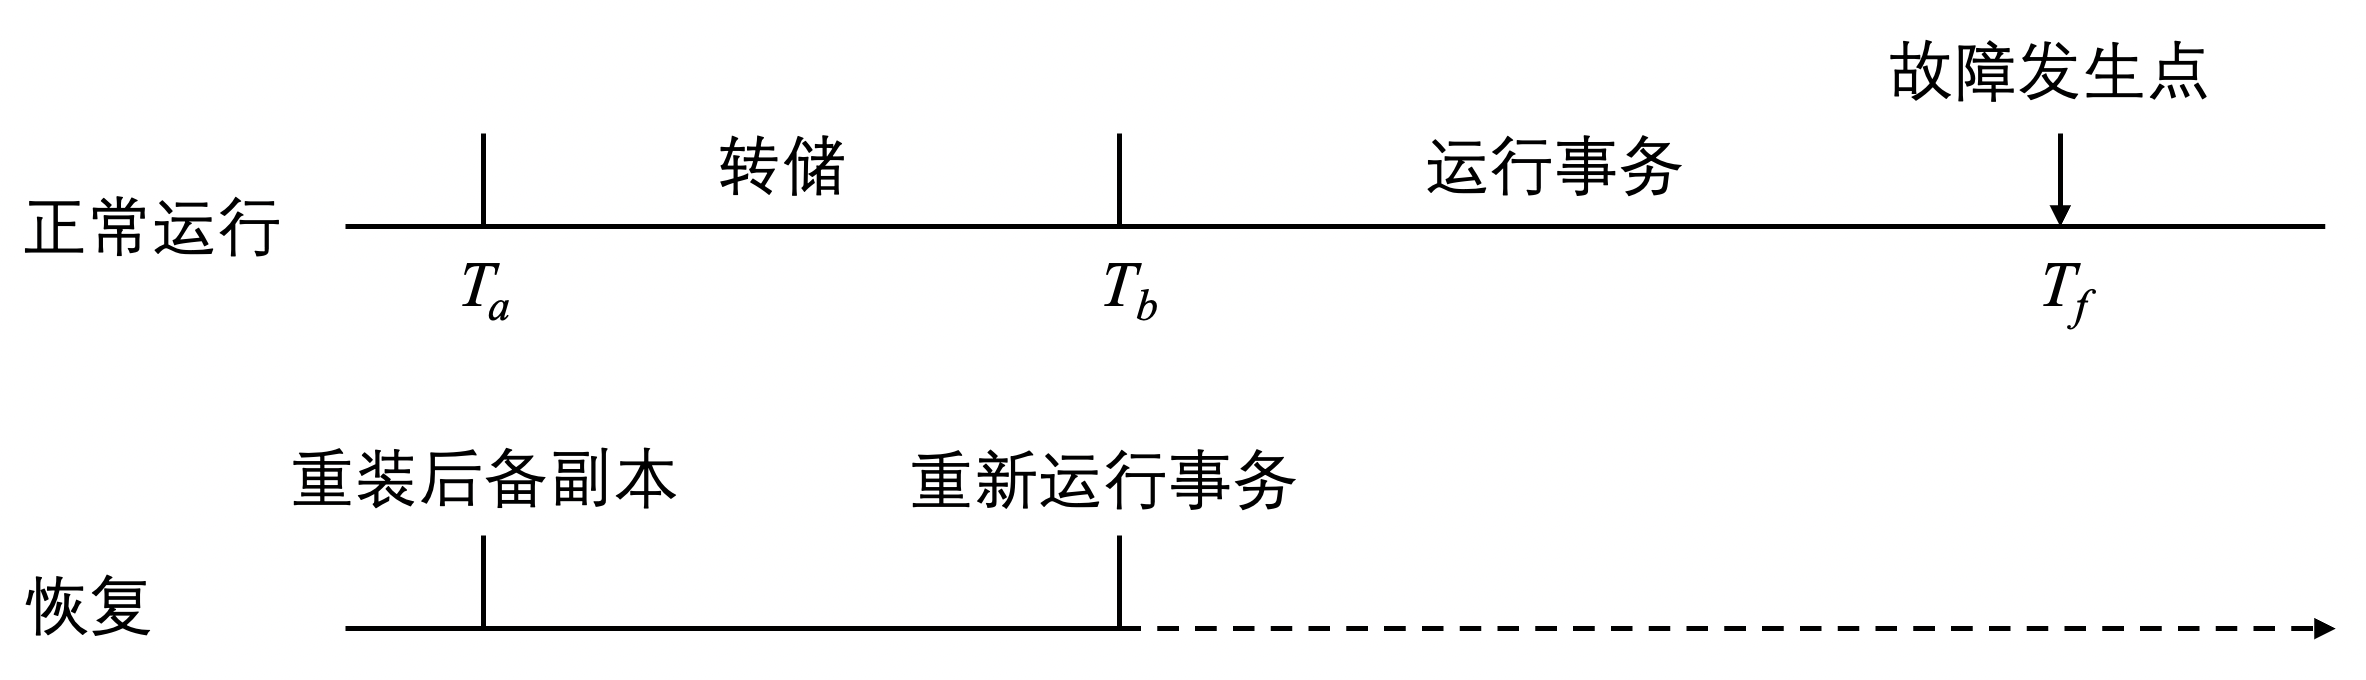
\includegraphics[width=0.65\textwidth]{images/10.1}
    \vspace{-1em}
\end{figure}

转储可分为静态转储和动态转储
\begin{itemize}
    \item 静态转储
    \begin{itemize}
        \item 在系统中无运行事务时进行的转储操作
        \item 转储开始时数据库处于一致性状态
        \item 转储期间不允许对数据库的任何存取、修改活动
        \item 得到的一定是一个数据一致性的副本    
        \item 优点:实现简单  
        \item 缺点:降低了数据库的可用性
        \begin{itemize}
            \item 转储必须等待正运行的用户事务结束
            \item 新的事务必须等转储结束
        \end{itemize}
    \end{itemize}
    \item 动态转储
    \begin{itemize}
        \item 转储操作与用户事务并发进行
        \item 转储期间允许对数据库进行存取或修改
        \item 优点
        \begin{itemize}
            \item 不用等待正在运行的用户事务结束
            \item 不会影响新事务的运行
        \end{itemize}
        \item 缺点:转储结束时后援副本上的数据并不能保证正确有效
        \item 利用动态转储得到的副本进行故障恢复
        \begin{itemize}
            \item 需要把动态转储期间各事务对数据库的修改活动登记下来,建立日志文件
            \item 后备副本加上日志文件就能把数据库恢复到某一时刻的正确状态
        \end{itemize}
    \end{itemize}
\end{itemize}

转储还可以分为海量转储和增量转储
\begin{itemize}
    \item 海量转储:每次转储全部数据库
    \item 增量转储:只转储上次转储后更新过的数据
    \item 海量转储与增量转储比较
    \begin{itemize}
        \item 从恢复角度看,使用海量转储得到的后备副本进行恢复往往更方便
        \item 如果数据库很大,事务处理又十分频繁,则增量转储方式更实用更有效
    \end{itemize}
\end{itemize}

\subsection{登记日志文件}

\subsubsection{日志文件的格式和内容}
日志文件是用来记录事务对数据库的更新操作的文件,日志文件主要有两种格式:以记录为单位的日志文件和以数据块为单位的日志文件
\begin{itemize}
    \item 对于以记录为单位的日志文件,日志文件中需要登记的记录包括
    \begin{itemize}
        \item 各个事务的开始标记(\verb|BEGIN TRANSACTION|)
        \item 各个事务的结束标记(\verb|COMMIT|\ 或\sverb|ROLLBACK|)
        \item 各个事务的所有更新操作
        \item 上述三个内容均作为日志文件的一个日志记录,每个日志记录的主要内容包括
        \begin{itemize}
            \item 事务标识(标明是哪个事务) 
            \item 操作类型(插入、删除或修改)
            \item 操作对象(记录内部标识)
            \item 更新前数据的旧值(对插入操作而言,此项为空值)
            \item 更新后数据的新值(对删除操作而言,此项为空值)
        \end{itemize}
    \end{itemize}
    \item 对于以数据块为单位的日志文件,每条日志记录的内容包括事务标识和被更新的数据块
\end{itemize}

\subsubsection{日志文件的作用}
\begin{itemize}
    \item 事务故障恢复和系统故障恢复必须用日志文件
    \item 在动态转储方式中必须建立日志文件,后备副本和日志文件结合起来才能有效地恢复数据库 
    \item 在静态转储方式中,也可以建立日志文件
    \begin{itemize}
        \item 当数据库毁坏后可重新装入后援副本把数据库恢复到转储结束时刻的正确状态
        \item 利用日志文件,把已完成的事务进行重做处理
        \item 对故障发生时尚未完成的事务进行撤销处理
        \item 不必重新运行那些已完成的事务程序就可把数据库恢复到故障前某一时刻的正确状态
    \end{itemize}
\end{itemize}

\begin{figure}[H]
    \vspace{-0.5em}
	\centering
	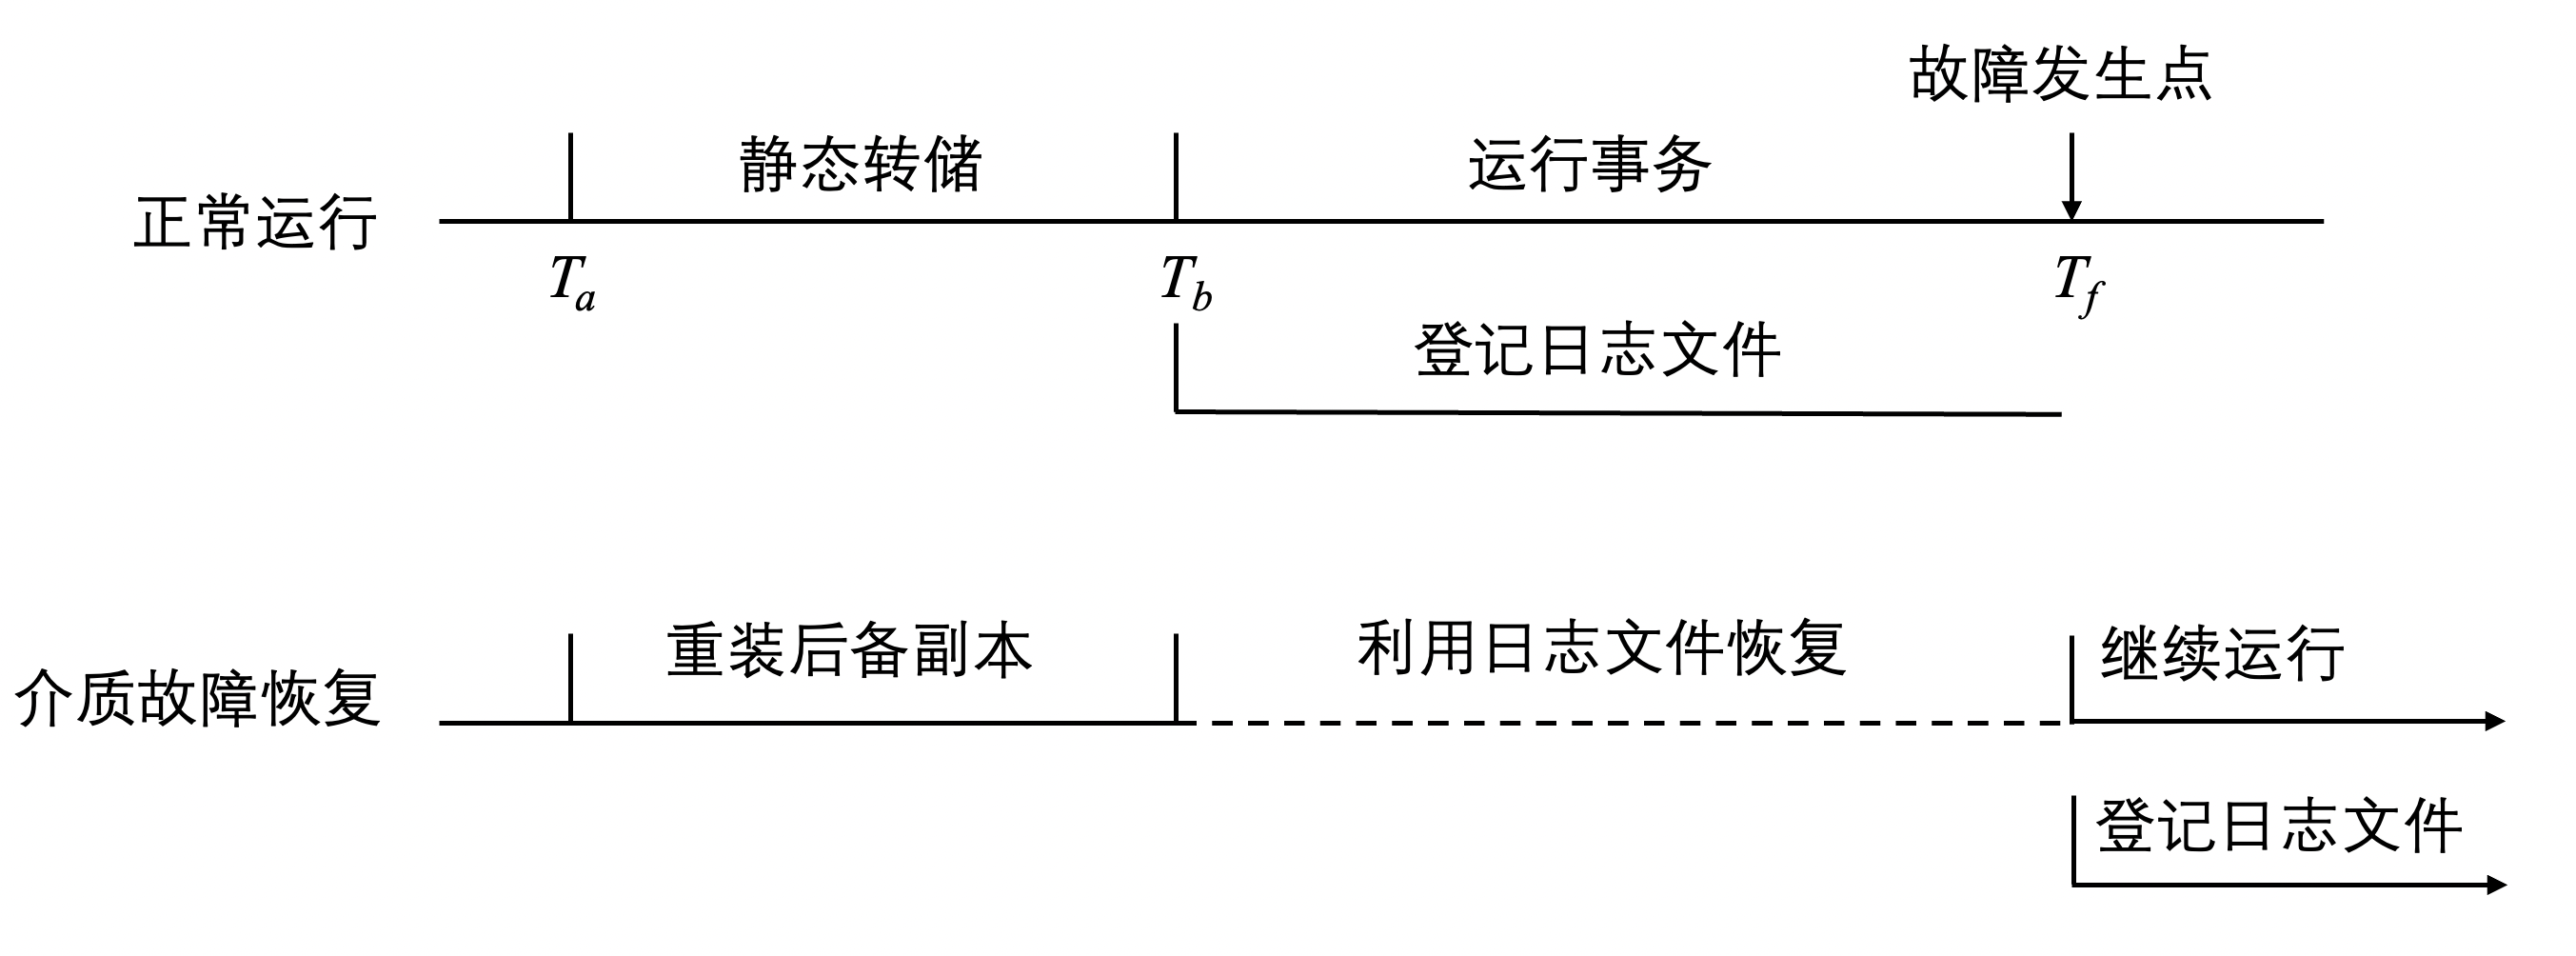
\includegraphics[width=0.65\textwidth]{images/10.2}
    \vspace{-1em}
\end{figure}

\subsubsection{登记日志文件}
为保证数据库是可恢复的,登记日志文件时必须遵循两条原则
\begin{itemize}
    \item 登记的次序严格按并发事务执行的时间次序
    \item 必须先写日志文件,后写数据库
    \begin{itemize}
        \item 写日志文件操作:把表示这个修改的日志记录写到日志文件中
        \item 写数据库操作:把对数据的修改写到数据库中
    \end{itemize}
\end{itemize}

先写日志文件的原因:
\begin{itemize}
    \item 写数据库和写日志文件是两个不同的操作
    \item 在这两个操作之间可能发生故障
    \item 如果先写了数据库修改,而在日志文件中没有登记下这个修改,则以后就无法恢复这个修改了
    \item 如果先写日志,但没有修改数据库,按日志文件恢复时只不过是多执行一次不必要的 UNDO 操作,并不会影响数据库的正确性
\end{itemize}

\section{恢复策略}

\subsection{事务故障的恢复}
事务故障:事务在运行至正常终止点前被终止
\begin{itemize}
    \item 恢复方法:由恢复子系统利用日志文件撤消(UNDO)此事务已对数据库进行的修改
    \item 事务故障的恢复由系统自动完成,对用户是透明的,不需要用户干预
\end{itemize}

事务故障的恢复步骤:
\begin{itemize}
    \item 反向扫描文件日志(即从最后向前扫描日志文件),查找该事务的更新操作
    \item 对该事务的更新操作执行逆操作。即将日志记录中“更新前的值”写入数据库
    \begin{itemize}
        \item 插入操作,“更新前的值”为空,则相当于做删除操作
        \item 删除操作,“更新后的值”为空,则相当于做插入操作
        \item 若是修改操作,则相当于用修改前值代替修改后值 
    \end{itemize}
    \item 继续反向扫描日志文件,查找该事务的其他更新操作,并做同样处理
    \item 如此处理下去,直至读到此事务的开始标记,事务故障恢复就完成了
\end{itemize}

\subsection{系统故障的恢复}
系统故障造成数据库不一致状态的原因
\begin{itemize}
    \item 未完成事务对数据库的更新可能已写入数据库
    \item 已提交事务对数据库的更新可能还留在缓冲区没来得及写入数据库
\end{itemize}

恢复方法:
\vspace{-0.8em}
\begin{multicols}{2}
    \begin{itemize}
        \item Undo故障发生时未完成的事务
        \item Redo已完成的事务
    \end{itemize}
\end{multicols}
\vspace{-1em}

系统故障的恢复由系统在重新启动时自动完成,不需要用户干预

系统故障的恢复步骤:
\begin{itemize}
    \item 正向扫描日志文件(即从头扫描日志文件)
    \begin{itemize}
        \item 重做(REDO) 队列:在故障发生前已经提交的事务。这些事务既有\sverb|BEGIN TRANSACTION|\ 记录,也有\sverb|COMMIT|\ 记录。
        \item 撤销 (UNDO)队列:故障发生时尚未完成的事务。这些事务只有\sverb|BEGIN TRANSACTION|\ 记录,无相应的\sverb|COMMIT|\ 记录。
    \end{itemize}
    \item 对撤销(UNDO)队列事务进行撤销(UNDO)处理
    \begin{itemize}
        \item 反向扫描日志文件,对每个撤销事务的更新操作执行逆操作
        \item 即将日志记录中“更新前的值”写入数据库 
    \end{itemize}
    \item 对重做(REDO)队列事务进行重做(REDO)处理
    \begin{itemize}
        \item 正向扫描日志文件,对每个重做事务重新执行登记的操作
        \item 即将日志记录中“更新后的值”写入数据库 
    \end{itemize}
\end{itemize}

\subsection{介质故障的恢复}
\begin{itemize}
    \item 介质故障的恢复的工作
    \vspace{-0.8em}
    \begin{multicols}{2}
        \begin{itemize}
            \item 重装数据库
            \item 重做已完成的事务
        \end{itemize}
    \end{multicols}
    \vspace{-1em}
    \item 介质故障的恢复需要数据库管理员介入
    \item 数据库管理员的工作
    \begin{itemize}
        \item 重装最近转储的数据库副本和有关的各日志文件副本
        \item 执行系统提供的恢复命令
    \end{itemize}
    \item 具体的恢复操作仍由数据库管理系统完成
\end{itemize}

介质故障的恢复步骤:
\begin{itemize}
    \item 装入最新的后备数据库副本(离故障发生时刻最近的转储副本),使数据库恢复到最近一次转储时的一致性状态
    \begin{itemize}
        \item 对于静态转储的数据库副本,装入后数据库即处于一致性状态
        \item 对于动态转储的数据库副本,还须同时装入转储时刻的日志文件副本,利用恢复系统故障的方法(即REDO+UNDO),才能将数据库恢复到一致性状态
    \end{itemize}
    \item 装入有关的日志文件副本(转储结束时刻的日志文件副本),重做已完成的事务
    \begin{itemize}
        \item 首先扫描日志文件,找出故障发生时已提交的事务的标识,将其记入重做队列
        \item 然后正向扫描日志文件,对重做队列中的所有事务进行重做处理。即将日志记录中“更新后的值”写入数据库
    \end{itemize}
\end{itemize}

\subsection{具有检查点的恢复技术}
\begin{itemize}
    \item 在日志文件中增加检查点记录
    \item 增加重新开始文件
    \item 恢复子系统在登录日志文件期间动态地维护日志
\end{itemize}

\subsubsection{检查点技术}
检查点记录的内容
\begin{itemize}
    \item 建立检查点时刻所有正在执行的事务清单
    \item 这些事务最近一个日志记录的地址
\end{itemize}

重新开始文件的内容
\begin{itemize}
    \item 记录各个检查点记录在日志文件中的地址
\end{itemize}

\begin{figure}[H]
    \vspace{-0.5em}
	\centering
	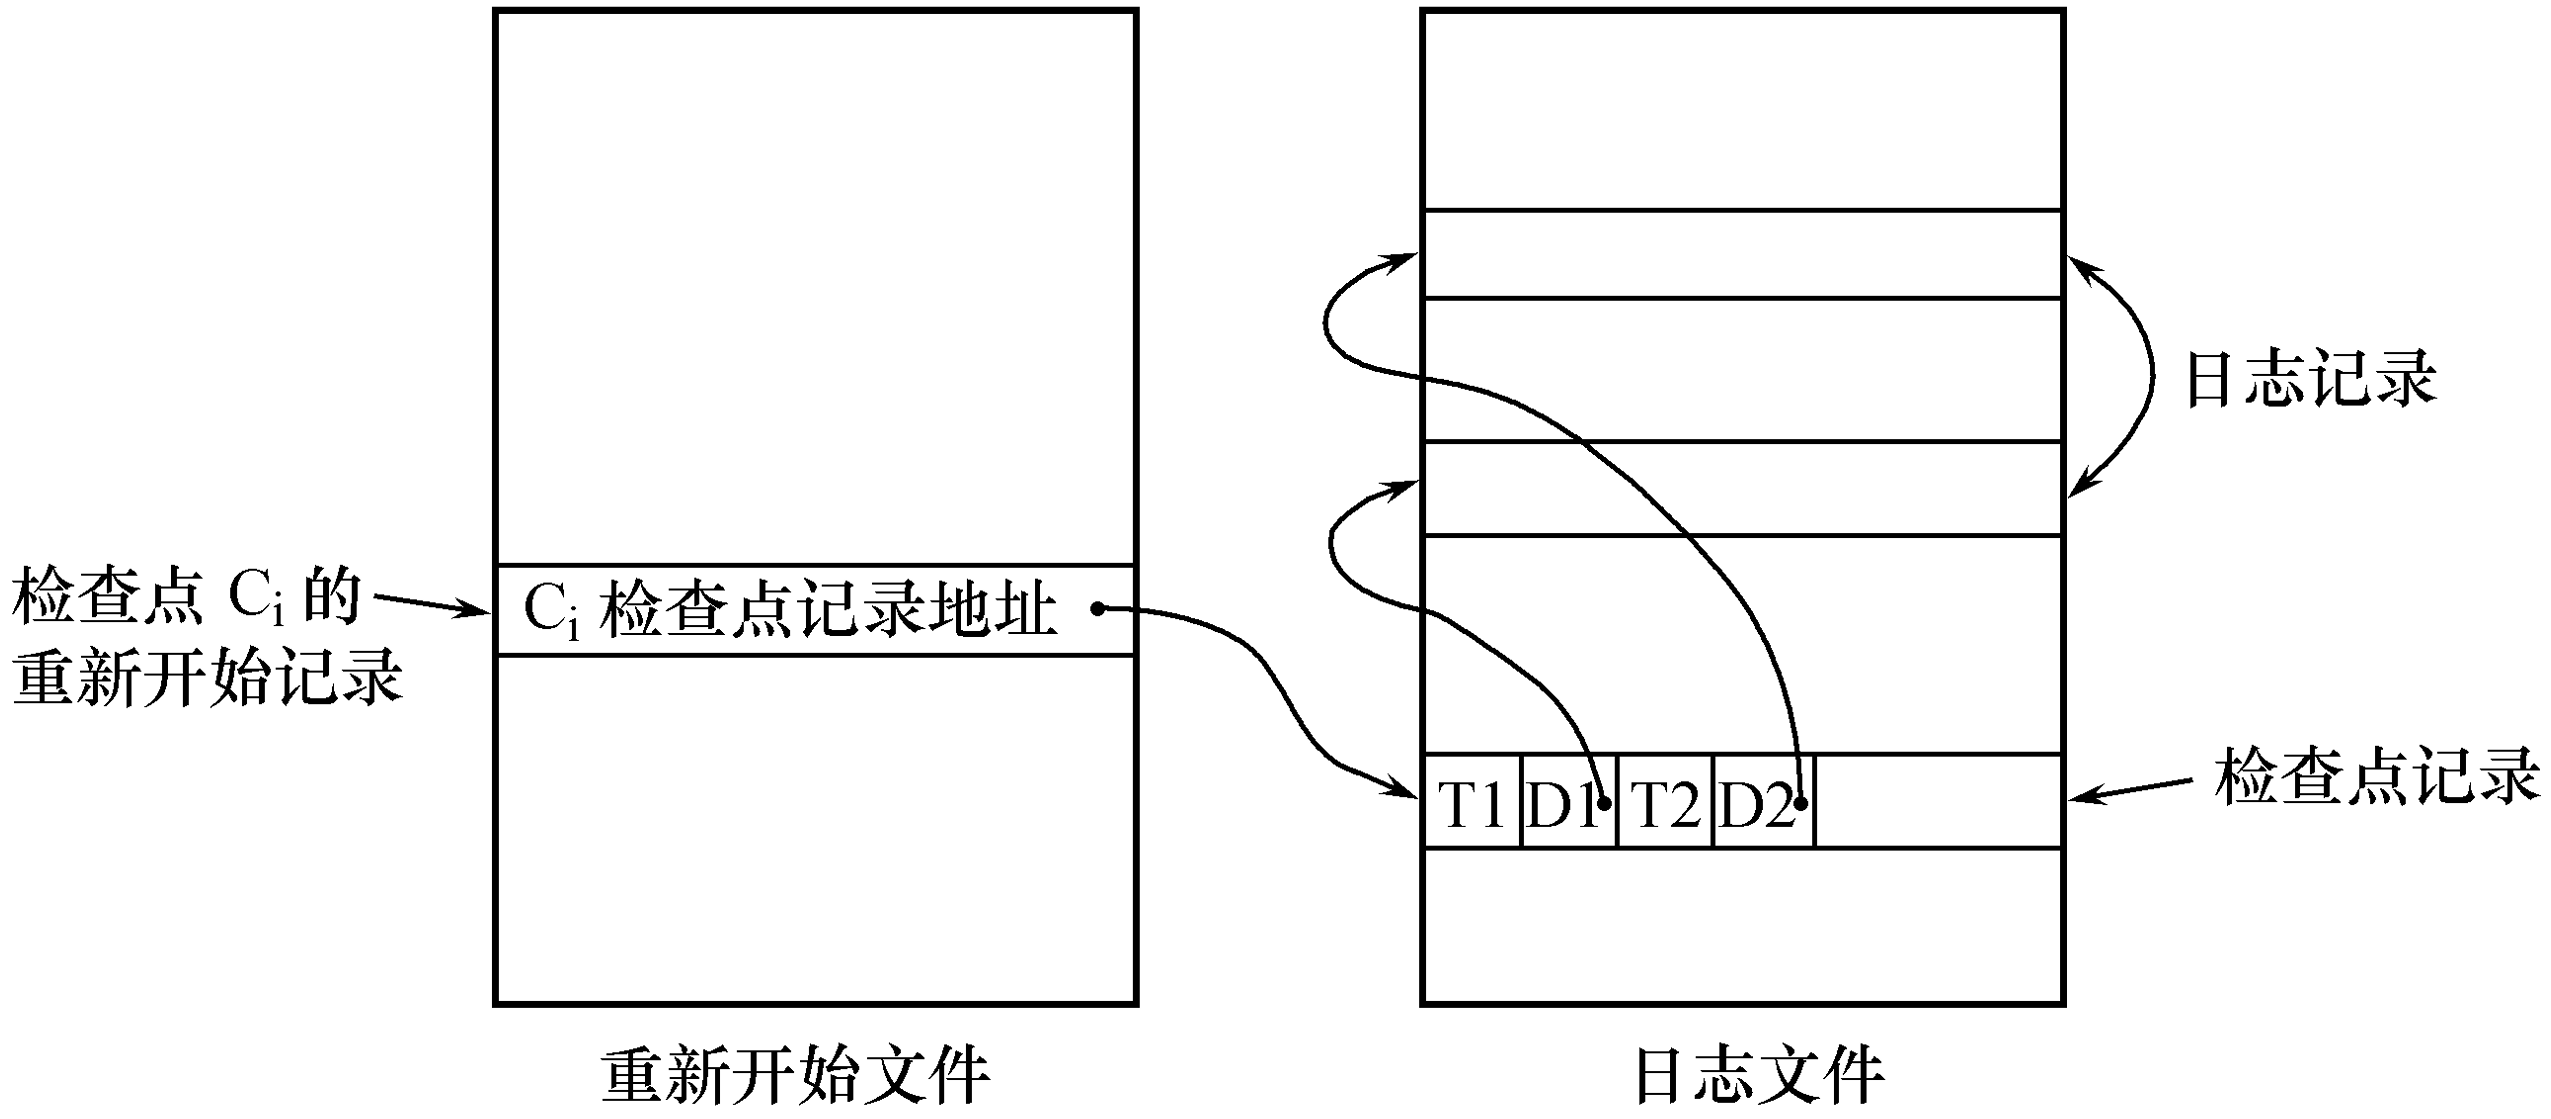
\includegraphics[width=0.5\textwidth]{images/10.5.4.1}
    \vspace{-1em}
\end{figure}

动态维护日志文件的方法:周期性地执行建立检查点,保存数据库状态操作
\begin{itemize}
    \item 将当前日志缓冲区中的所有日志记录写入磁盘的日志文件上
    \item 在日志文件中写入一个检查点记录
    \item 将当前数据缓冲区的所有数据记录写入磁盘的数据库中
    \item 把检查点记录在日志文件中的地址写入一个重新开始文件
\end{itemize}

\subsubsection{利用检查点的恢复策略}
系统出现故障时,恢复子系统将根据事务的不同状态采取不同的恢复策略 
\begin{figure}[H]
    \vspace{-0.5em}
	\centering
	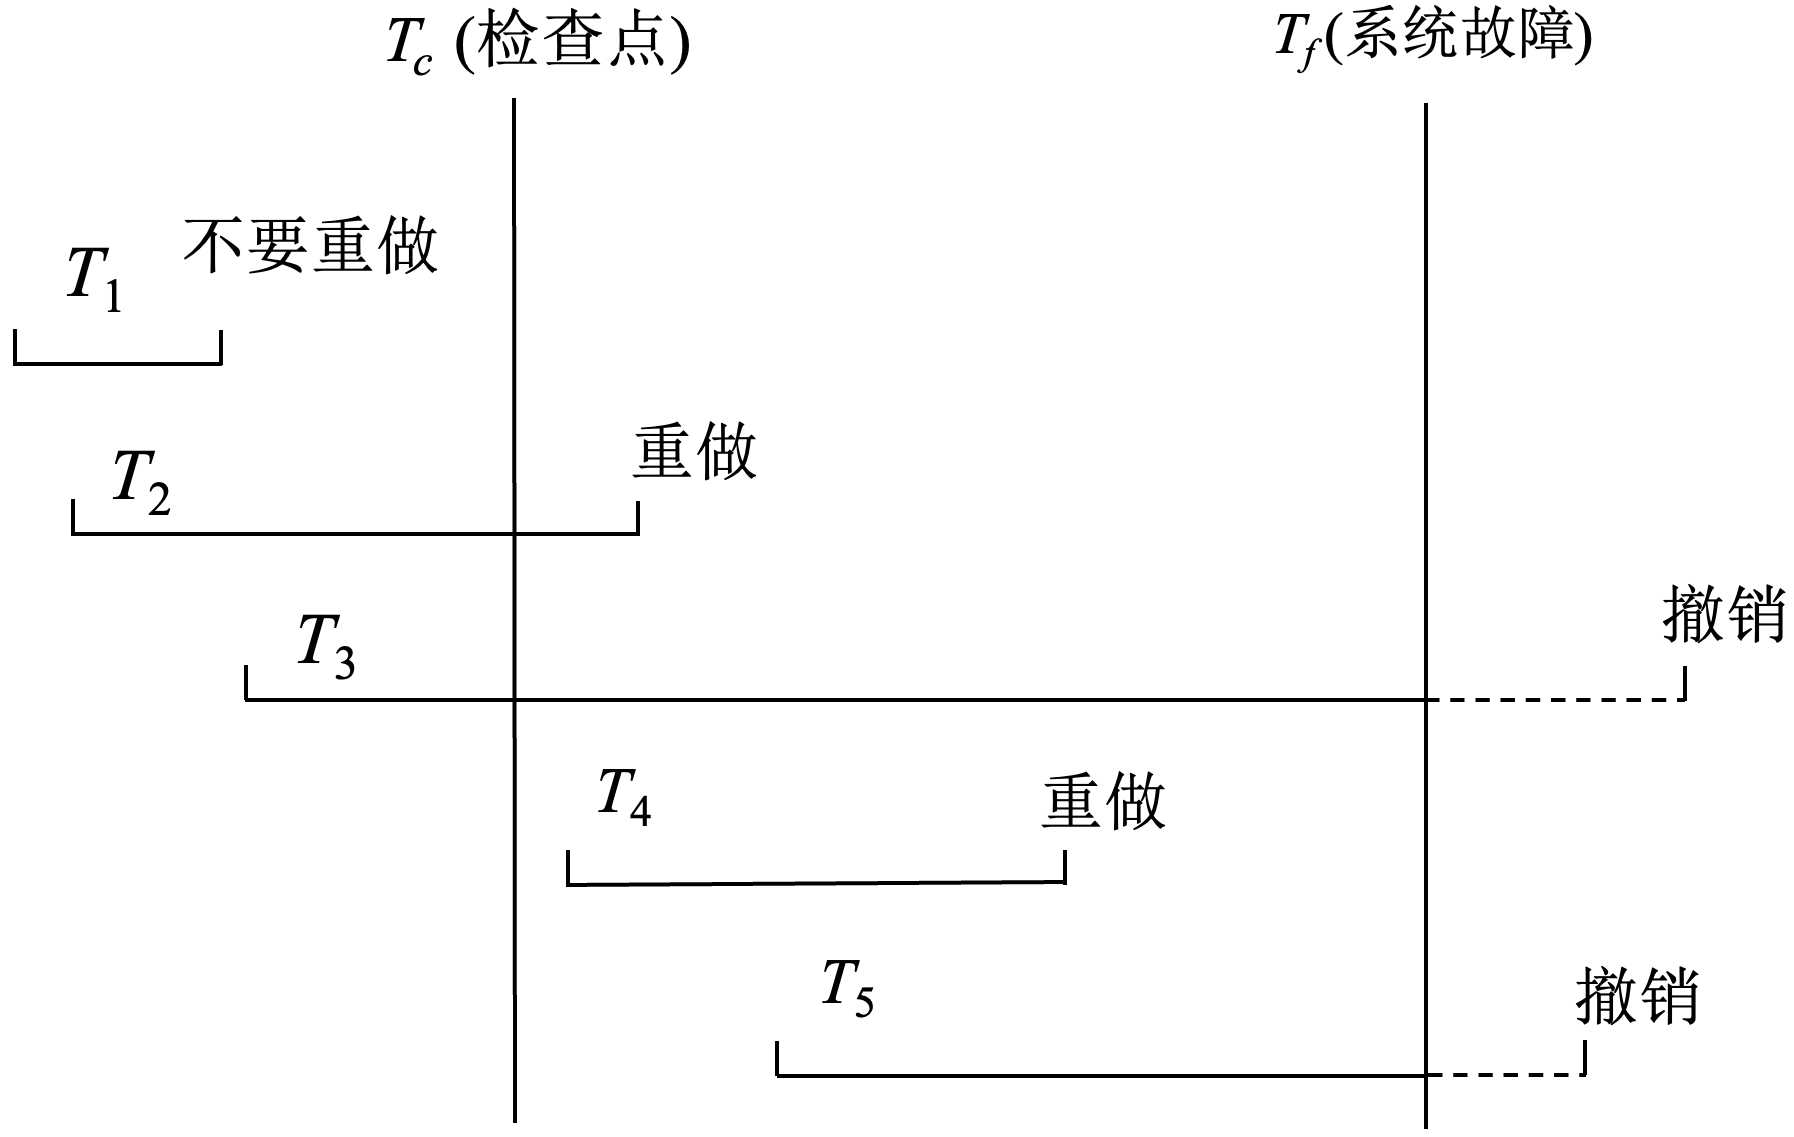
\includegraphics[width=0.5\textwidth]{images/10.5.4.2}
    \vspace{-1em}
\end{figure}
\begin{itemize}
    \item 从重新开始文件中找到最后一个检查点记录在日志文件中的地址,由该地址在日志文件中找到最后一个检查点记录
    \item 由该检查点记录得到检查点建立时刻所有正在执行的事务清单ACTIVE-LIST
    \begin{itemize}
        \item 建立两个事务队列:UNDO-LIST和UNDO-LIST
        \item 把ACTIVE-LIST暂时放入UNDO-LIST队列,REDO队列暂为空
    \end{itemize}
    \item 从检查点开始正向扫描日志文件,直到日志文件结束
    \begin{itemize}
        \item 如有新开始的事务$T_i$,把$T_i$暂时放入UNDO-LIST队列
        \item 如有提交的事务$T_j$,把$T_j$从UNDO-LIST队列移到REDO-LIST队列;直到日志文件结束
    \end{itemize}
    \item 对UNDO-LIST中的每个事务执行UNDO操作
    \item 对REDO-LIST中的每个事务执行REDO操作
\end{itemize}

	
	% \begin{figure}[H]
    % \vspace{-0.5em}
	% \centering
	% \includegraphics[width=0.4\textwidth]{images/}
    % \vspace{-1em}
	% \end{figure}

	% \vspace{-0.8em}
	% \begin{multicols}{2}
    % \begin{itemize}
    %     \item 
    % \end{itemize}
	% \end{multicols}
	% \vspace{-1em}


\end{document}


